\documentclass[a4paper,oneside,12pt]{book}
%----------------------------------------------------------------------------------------
%	COVER PAGE
%   The cover page is laid out in title/title.tex. You can choose a colour
%   or black and white logo
%----------------------------------------------------------------------------------------

%----------------------------------------------------------------------------------------
%	THESIS INFORMATION
%   Put title, author name, degree, type of work, school, department in here
%   It will be used for the title page and for the embedded PDF information
%----------------------------------------------------------------------------------------

\newcommand{\thesistitle}{HubSpot Software Engineering Internship} % Your thesis title, this is used in the title and abstract
\newcommand{\degree}{MAI (Computer Engineering)} % Your degree name, this is used in the title page and abstract
\newcommand{\typeofthesis}{Internship Report} % dissertation, Final Year Project, report, etc.
\newcommand{\authorname}{Stefano Lupo} % Your name, this is used in the title page and PDF stuff
%% Comment out the next line if you don't want your ID to appear
\newcommand{\authorid}{14334933} % Your ID
\newcommand{\keywords}{HubSpot, Software Engineering, Programming, Computer Engineering, 4E4 Internship} % Keywords for your thesis
\newcommand{\school}{\href{http://www.scss.tcd.ie}{School of Computer Science and Statistics}} % Your school's name and URL, this is used in the title page

%% Custom commands
\newcommand{\team}{Email Sending Infrastructure}

%% Comment out the next line if you don't want a department to appear
%\newcommand{\department}{\href{http://researchgroup.university.com}{Department Name}} % Your research group's name and URL, this is used in the title page

\AtBeginDocument{
\hypersetup{pdftitle=\thesistitle} % Set the PDF's title to your title
\hypersetup{pdfauthor=\authorname} % Set the PDF's author to your name
\hypersetup{pdfkeywords=\keywords} % Set the PDF's keywords to your keywords
\hypersetup{pdfsubject=\degree} % Set the PDF's keywords to your keywords
}

%% Language and font encodings
\usepackage[T1]{fontenc} 
\usepackage[utf8]{inputenc}
\usepackage[english]{babel}

%% Bibliographical stuff
\usepackage[round,sort,comma,numbers]{natbib}

%% Document size
% include showframe as an option if you want to see the boxes
\usepackage[a4paper,top=2.54cm,bottom=2.54cm,left=2.54cm,right=2.54cm,headheight=16pt]{geometry}

%% Useful packages
\usepackage{amsmath}
\usepackage[autostyle=true]{csquotes} % Required to generate language-dependent quotes in the bibliography
\usepackage[pdftex]{graphicx}
\usepackage[colorinlistoftodos]{todonotes}
\usepackage[colorlinks=true, allcolors=black]{hyperref}
\usepackage{caption} % if no caption, no colon
\usepackage{sfmath} %use sans-serif in the maths sections too
\usepackage[parfill]{parskip}    % Begin paragraphs with an empty line rather than an indent
\usepackage{setspace} % to permit one-and-a-half or double spacing
\usepackage{enumerate} % fancy enumerations like (i) (ii) or (a) (b) and suchlike
\usepackage{booktabs} % To thicken table lines
\usepackage{fancyhdr}

%% My Packages
\usepackage{enumitem} %Nested lists a la TOC
\setlist[enumerate]{label*=\arabic*.}
\usepackage{scrextend} % labeling lists

\pagestyle{plain} % Embrace simplicity!


%% It is not a requirement of the university that the font should be sans-serif, but
%% the Mechanical engineers require it. Comment out the following line to disable it
\renewcommand{\familydefault}{\sfdefault} %use the sans-serif font as default

%% If you're not using sans-serif, consider using Palatino instead of the LaTeX standard
%\usepackage{mathpazo} % Use the Palatino font by default if you prefer it to Computer Modern

\renewcommand{\theequation}{\arabic{equation}} %% use continuous equation numbers

%% Format Chapter headings appropriately
\usepackage{titlesec}
\titleformat{\chapter}[hang] 
{\normalfont\huge\bfseries}{\thechapter}{1cm}{} 

\title{\thesistitle}
\author{\authorname}

\frontmatter
\begin{document}
\begin{titlepage}

\center % Center everything on the page

%% All the text parameters should be taken from the start of the main.tex file.
%% You should only alter stuff here if you want to change the layout

%----------------------------------------------------------------------------------------
%	LOGO SECTION
%----------------------------------------------------------------------------------------
%% Choose one of the following -- a colour or black-and-white logo


\includegraphics{title/Trinity_RGB_transparent_main.png}\\[1cm] 
%
\includegraphics[width=12cm]{title/black-stacked-trinity.jpg}\\[1cm] 

\Large \school\\[1.5cm] % Minor heading such as course title
\ifdefined\department
\large \department\\[1.5cm] % Minor heading such as course title
\fi

%----------------------------------------------------------------------------------------
%	TITLE SECTION
%----------------------------------------------------------------------------------------
\makeatletter
{ \huge \bfseries \thesistitle}\\[1.5cm] % Title of your document
 

%----------------------------------------------------------------------------------------
%	AUTHOR SECTION
%----------------------------------------------------------------------------------------

\ifdefined\authorid
\authorname\\ % Your name
\authorid\\[2cm] % Your Student ID
\else
\authorname\\[2cm] % Your name
\fi

%----------------------------------------------------------------------------------------
%	DATE SECTION
%----------------------------------------------------------------------------------------

{\large \today}\\[2cm] % Date, change the \today to a set date if you want to be precise

 
%----------------------------------------------------------------------------------------
%	TYPE OF THESIS SECTION
%----------------------------------------------------------------------------------------
 A \typeofthesis\ submitted in partial fulfilment\\of the requirements for the degree of\\
\degree

\vfill % Fill the rest of the page with whitespace

\end{titlepage}
\pagenumbering{roman}
\section*{\Huge{Declaration}}
\vspace{1cm}
I hereby declare that this project is entirely my own work and that it has not been submitted as an exercise for a degree at this or any other university.

\vspace{1cm}
I have read and I understand the plagiarism provisions in the General Regulations of the University Calendar for the current year, found at \url{http://www.tcd.ie/calendar}.
\vspace{1cm}

I have also completed the Online Tutorial on avoiding plagiarism `Ready Steady Write', located at
\url{http://tcd-ie.libguides.com/plagiarism/ready-steady-write}.
\vspace{3cm}

Signed:~\rule{5cm}{0.3pt}\hfill Date:~\rule{5cm}{0.3pt}

\chapter*{Abstract}
A short summary of the problem investigated, the approach taken and the key findings. This should be around 400 words, or less.

This should be on a separate page.

DESCRIBE THE FOLLOWING LEARNING OUTCOMES (throughout the report, not the abstract)
\begin{enumerate}
	\item contribute to the design and development of systems at forefront of CS research and evaluate their performance
	\item apply theoretical knowledge to solve real world problems
	\item practice and further devel skills in comms, mgmt and teamwork
	\item practice and further develop skills in time management and reporting
	\item contribute to an ethical and profesional work culture
\end{enumerate}

\begin{enumerate}
	\item 
\end{enumerate}

\newpage
\onehalfspacing\raggedright %\raggedright turns off justification and hypenation

\section*{\Huge{Acknowledgements}}
Thanks Mum!

You should acknowledge any help that you have received (for example from technical staff), or input provided by, for example, a company.
\tableofcontents
\listoffigures
\listoftables
\newpage
\section*{\Huge{Nomenclature}}
\begin{tabular}{lp{9cm}l}
A&Area of the wing&$m^{2}$\\
B\\
C& Roman letters first, with capitals\ldots\\
a&then lower case.\\
b\\
c\\
$\Gamma$&Followed by Greek capitals\ldots\\
$\alpha$&then lower case greek symbols.\\
$\beta$\\
$\epsilon$\\
TLA&Finally, three letter acronyms and other abbreviations arranged alphabetically\\
\end{tabular}
\vspace{2cm}

If a parameter has a typical unit that is used throughout your report, then it should be included here on the right hand side.

If you have a very mathematical report, then you may wish to divide the nomenclature list into functions and variables, and then sub- and super-scripts.

Note that Roman mathematical symbols are typically in a serif font in italics.

\mainmatter


\begin{enumerate}
	\item Introduction (5 Pages)
	\begin{enumerate}
    	\item Who are HubSpot - 2
        \item The Email Sending Infrastructure Team - 2
        \item Goals of the team or something - 1
    \end{enumerate}
    
    \item Technologies Used (~26 pages, probably excessive)
    \begin{enumerate}
    	\item Java 8 Features (streams, CF, lambdas, Executors) - 5
        \item Kafka - 5
        \item Hadoop - 3
        \item DNS - 3
        \item SMTP - 2
        \item MySql (InnoDB) - 3
        \item HBase (Sync, Idempot, Locks) - 3
        \item ZooKeeper (+ Circus) - 2
        \item RateLimiters, Distributed RateLimiters
    \end{enumerate}
    
    \item HubSpot Methodology (10 Pages)
    \begin{enumerate}
    	\item Java MicroServices - 5
        \item React Native / Redux front end - 4
    \end{enumerate}
    
    \item Major Projects Undertaken (20)
    \begin{enumerate}
    	\item Rebuilt DNS management - 5
        \item Auto DNS for dedicated accounts - 5
    	\item EmailMtaSending Kafka stuff - 5
    \end{enumerate}
    
\end{enumerate}

\chapter{Introduction}
This document 

\section{Fonts, sizes, justification}

Throughout the document, a sans-serif font should be used. The font size should be 12 pt for main text. The text should be left justified and without hyphenation. Avoid italics and boldface in the main text. These font requirements comply with TCD policy on accessibility.

The page number should appear at the bottom of each page starting at 1 on the first page of the Introduction chapter. 

\section{Headings of sections and subsections}
Chapters should be divided into appropriate subsections. The section should be numbered sequentially from 1 within each chapter (e.g. 1.1, 1.2, 1.3 etc.).

\subsection{Subsection name style}
The subsections if used should be numbered sequentially within each section. You should really try to avoid using subsubsections, but if you do they should not be numbered.

\subsubsection*{Subsection}
This is a subsection. The asterisk after the command means it won't be printed with a number.

\subsection{Length of the report}
The page margins are set to 2.54 cm top, bottom, left and right. There may be a table or figure for which it is sensible to deviate from these margins, but in general the main text should be formatted within the specified margins.

The body of the report should be organized into several chapters. There are a number of chapters that you must have: an introduction; a background or literature review chapter; and a conclusion chapter. The focus of the other chapters will depend on your specific project.

The body of the report must be no more 60 pages for MAI. This does not include the front matter, references list and any appendices. In other words, from the first page of the Introduction to the last page of the Conclusions chapters must be less than 60 pages for MAI.

If you exceed these page limits or deviate significantly from this format, you will lose marks.

\section{Contents of the Introduction}
The introduction presents the nature of the problem under consideration, the context of the problem to the wider field and the scope of the project. The objectives of the project should be clearly stated.

\section{Contents of the background chapter}
The second chapter is typically a literature review, or survey of the state of the art, or a detailed assessment of the context and background for the project. The exact nature of this chapter depends on the topic and/or methods of the project. It is essential that the work of other people is properly cited. This will be discussed in detail in chapter 2 below. Note that you should use references wherever is appropriate through the report, not just in the literature review chapter.

\section{The Conclusions chapter}
The final chapter should give a short summary of the key methods, results and findings in your project. You should also briefly identify what, if any, future work might be executed to resolve unanswered questions or to advance the study beyond the scope that you identified in Chapter 1.

\chapter{Tasks Undertaken}


Throughout the course of the internship, a variety these tasks were undertaken and completed.  

For the sake of brevity a small subset of the most interesting of these tasks are outlined below. 


\chapter{Figures, Tables and Referencing}

\section{Figures}
Graphs, pictures and other images should be included in your report as a numbered, captioned figure. An example is given in Figure \ref{veldis}.

%%%%%%%%%%%%%%%%%%%%%%%%%%%%%%%%%%%%%%%%
\begin{figure}[h]
      \centering
      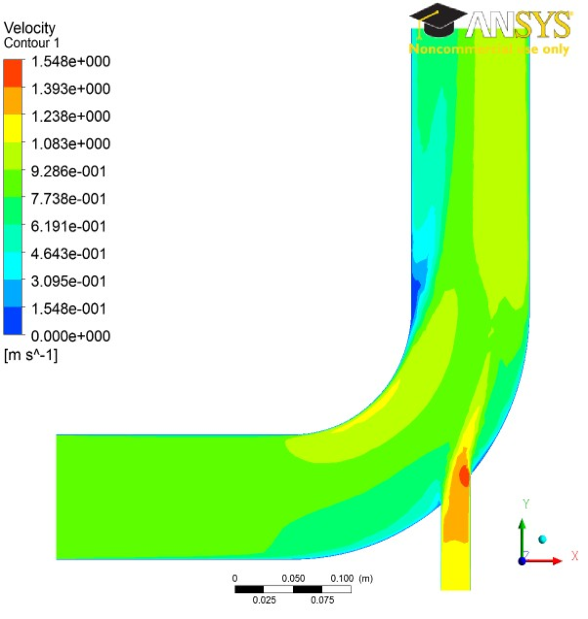
\includegraphics{background/5e1-1.pdf}
      \caption{Velocity distribution on the mid-plane for an inlet velocity for case 1.}
      \label{veldis}
\end{figure}
%%%%%%%%%%%%%%%%%%%%%%%%%%%%%%%%%%%%%%%%

The figure and caption should be centred. The figure numbering starts at 1 at the beginning of each chapter. The caption should provide a brief description of what is being shown. The figure should appear in the document after it is referred to in the text. No figure should be included which is not referred to in the text. Ensure that the size and resolution of images imported from software are sufficient to read any text.

\section{Tables}
Tables are an important way of displaying your results; Table \ref{tab:treatments} is a sample table, adapted from the Master/Doctoral Thesis template at \url{http://www.latextemplates.com/cat/theses}, which was generated with this code:

{\footnotesize
\begin{verbatim}
\begin{table}[b]
\caption{The effects of treatments X and Y on the four groups studied.}
\label{tab:treatments}
\centering
\begin{tabular}{l l l}
\toprule
\textbf{Groups} & \textbf{Treatment X} & \textbf{Treatment Y} \\\midrule
1 & 0.2 & 0.8\\
2 & 0.17 & 0.7\\
3 & 0.24 & 0.75\\
4 & 0.68 & 0.3\\
\bottomrule\\
\end{tabular}
\end{table}
\end{verbatim}
}

\begin{table}[b]
\caption{The effects of treatments X and Y on the four groups studied.}
\label{tab:treatments}
\centering
\begin{tabular}{l l l}
\toprule
\textbf{Groups} & \textbf{Treatment X} & \textbf{Treatment Y} \\
\midrule
1 & 0.2 & 0.8\\
2 & 0.17 & 0.7\\
3 & 0.24 & 0.75\\
4 & 0.68 & 0.3\\
\bottomrule\\
\end{tabular}
\end{table}

Tables are numbered in the same way as figures. Typically tables also have a short caption, but this is not universally true. The number and caption appear above the table, not below as with figures. Again, no table should appear in the report which has not been referred to in the text. Tables should come after they are discussed in the text. The exact formatting of the table depends somewhat on the content of the table, but in general, the text in the table should be the same font and size as the main text. 

\section{Equations}
All equations should be numbered sequentially. Do not restart the numbering at the beginning of each chapter. Unlike figures and tables, you may not need to refer to every equation in the text. You should take care to format equations properly. Do no simply try to use plain text. Use the equation layout facilities. An example of how equations should appear is shown in Equation \ref{sampleequation}. Here is the code for it:

{\footnotesize
\begin{verbatim}
\begin{equation}
\textrm{div}(\underline{u}) = \frac{\delta u}{\delta x} + \frac{\delta v}{\delta y} +
        \frac{\delta w}{\delta z} = 0
\label{sampleequation}
\end{equation} 
\end{verbatim}
}

\begin{equation}
\textrm{div}(\underline{u}) = \frac{\delta u}{\delta x} + \frac{\delta v}{\delta y} + \frac{\delta w}{\delta z} = 0
\label{sampleequation}
\end{equation} 

\section{Referencing published work}
It is important to give appropriate credit to other people for the work that they have shared through publications. In fact, you must sign a declaration in your report stating that you understand the nature of plagiarism. As well as avoiding plagiarism, citing results or data from the literature can strengthen your argument, provide a favourable comparison for your results, or even demonstrate how superior your work is.

There are many styles to reference published work. For example, the parenthetical style (which is also called the Harvard style) uses the author and date of publication (e.g. ``Smith and Jones, 2001''). There is also the Vancouver (or the citation sequence) style, which is shown in this document. In the Vancouver style, the publications are cited using a bracket number which refers to the list in the References section at the end of the report. The references are listed in order that they are cited in the report. A variant is name sequence style in which the publications are referenced by number, but the list is arranged alphabetically. For example, the text might say: several studies have examined the sound field around tandem cylinders generated by flow\cite{fitzpatrick2003flow,finnegan2010experimental}, while other investigations have focused on the effect of an applied sound field on the flow\cite{hall2003vortex}. Papers from conference proceedings\cite{jordan2001array}, books\cite{paidoussis2010fluid} and technical reports\cite{reyes2007power,iea2011} can be dealt with in the same style.

The Vancouver style has the advantage that it is a little more compact in the text and does not distract from the flow of the sentence if there are a lot of citations. However, it has the disadvantage that it is not immediately clear to the reader what particular work has been referenced.

It actually does not matter which particular referencing style is used as long as three important considerations are observed:
\begin{itemize}
\item the referencing style used throughout the document is consistent;
\item all material used or discussed in the text is properly cited;
\item nothing is included in the reference list that has not been cited.
\end{itemize}

This template has a suitable referencing style already set up -- you should use it and use the built-in BibTeX system to manage your references. See above for examples of how to cite a reference and look in the \texttt{sample.bib} file to see BibTeX references. Remember \href{http://scholar.google.com}{Google Scholar} and other search engines will give you BibTeX references for lots of academic publications. Otherwise, you can easily make up your own based on the examples in that file.
% \chapter{\LaTeX}
\label{latexchapter}
seeing \LaTeX{}, or more properly ``\LaTeXe{}'', is a very useful document processing program. It is very widely used, widely available, stable and free. Famously, \TeX, upon which \LaTeX{} is built, was originally developed by the eminent American mathematician Donald Knuth because he was tired of ugly mathematics books\cite{shustek2008interview}. Although it has a learning curve (made much less forbidding by online tools and resources -- see below), it allows the writer to concentrate more fully on the content, and takes care of most everything else.

While it can be used as a word processor, it is a \emph{typesetting} system, and Knuth's idea was that it could be used to produce beautiful looking books:
\begin{quote}
\emph{\LaTeX{} is a macro package which enables authors to typeset and print their work at the highest typographical quality, using a predefined, professional layout.}\footnote{This is from \citet{oetiker2001not}. Did we mention that you should minimise your use of footnotes?}
\end{quote}
\LaTeX{} has great facilities for setting out equations and a powerful and very widely supported bibliographic system called BibTeX, which takes the pain out of referencing.

Three useful online resources make \LaTeX~much better:
\begin{enumerate}
\item An excellent online \LaTeX{} environment called ``Overleaf'' is available at \url{http://www.overleaf.com} that runs in a modern web browser. It's got this template available -- search for a TCD template. Overleaf can work in conjunction with Dropbox, Google Drive and, in beta, GitHub.
\item Google Scholar, at \url{http://scholar.google.com}, provides BibTeX entries for most of the academic references it finds.
\item An indispensable and very fine introduction to using \LaTeX{} called \emph{``The not so short introduction to LATEX 2$\varepsilon$''} by \citet{oetiker2001not} is online at \url{https://doi.org/10.3929/ethz-a-004398225}. Browse it before you use \LaTeX~for the first time and  read it carefully when you get down to business.
\end{enumerate}
Other tools worth mentioning include:
\begin{itemize}
\item \texttt{Draw.io} -- an online drawing package that can output PDFs to Google Drive -- see \url{https://www.draw.io}.
\end{itemize}
\chapter{Evaluation}
\chapter{Conclusion}
\bibliographystyle{unsrtnat}
\bibliography{bibs/sample}
\appendix
\renewcommand{\thechapter}{A\arabic{chapter}}
\chapter{Appendix}
You may use appendices to include relevant background information, such as calibration certificates, derivations of key equations or presentation of a particular data reduction method. You should not use the appendices to dump large amounts of additional results or data which are not properly discussed. If these results are really relevant, then they should appear in the main body of the report.

\section{Appendix numbering}
Appendices are numbered sequentially, A1, A2, A3\ldots The sections, figures and tables within appendices are numbered in the same way as in the main text. For example, the first figure in Appendix A1 would be Figure A1.1. Equations continue the numbering from the main text.



\end{document}